\chapter{Part pràctica}

{\Large \textbf{Primer experiment}}
\newline

Vaig començar a organitzar-me i a buscar el material que hauria d’utilitzar per fer la part pràctica. La meva intenció era llegir una mica i complir un dels objectius que m’havia proposat per a l’estiu. No acostumo a llegir gaire; per això, si llegir per informar-me m’ajudava, ho feia amb molt de gust. Amb l’ajuda del meu tutor, Fernando, vaig trobar unes tires reactives a Amazon que em permetrien analitzar químicament l’aigua. Amb una sola tira es poden mesurar fins a setze paràmetres diferents. Aquestes tires tenien un cost de 19,99 euros. També disposava d’un mesurador digital de pH, cedit per l’institut, que considerava el material més fiable, ja que proporciona una lectura exacta i no un valor aproximat.

L’objectiu principal era determinar la concentració de diferents compostos en una mostra d’aigua concreta i comparar-ne els resultats amb les dades oficials disponibles. Abans de fer la comparació, primer necessitava extreure les meves pròpies dades. Gràcies al material que tenia, podia obtenir resultats per més d’una via i comparar entre si les dades obtingudes i les oficials. La raó de fer-ho de diverses maneres era avaluar quina era la més eficient i, si era possible, posar a prova la fiabilitat de les dades oficials mitjançant l’experimentació directa.

Tan bon punt em van arribar les tires, vaig iniciar els experiments. La primera prova va consistir a recollir aigua de l’aixeta de casa meva. Vaig utilitzar una ampolla buida per emmagatzemar-la. El pas següent era entendre el funcionament de les tires que havia comprat. L’únic inconvenient era que el pH es repetia en els dos metodes, per això vaig decidir mesurar-lo per les dues vies: amb les tires d’Amazon i amb el mesurador digital.

Gràcies a les explicacions de l’Àlex Tuca, vaig aprendre a utilitzar correctament el mesurador de pH. Segons les seves instruccions, un cop feta la mesura, calia netejar el dispositiu amb aigua destil·lada. Com que no en tenia, vaig anar-ne a comprar.
\begin{figure}[H]
\centering
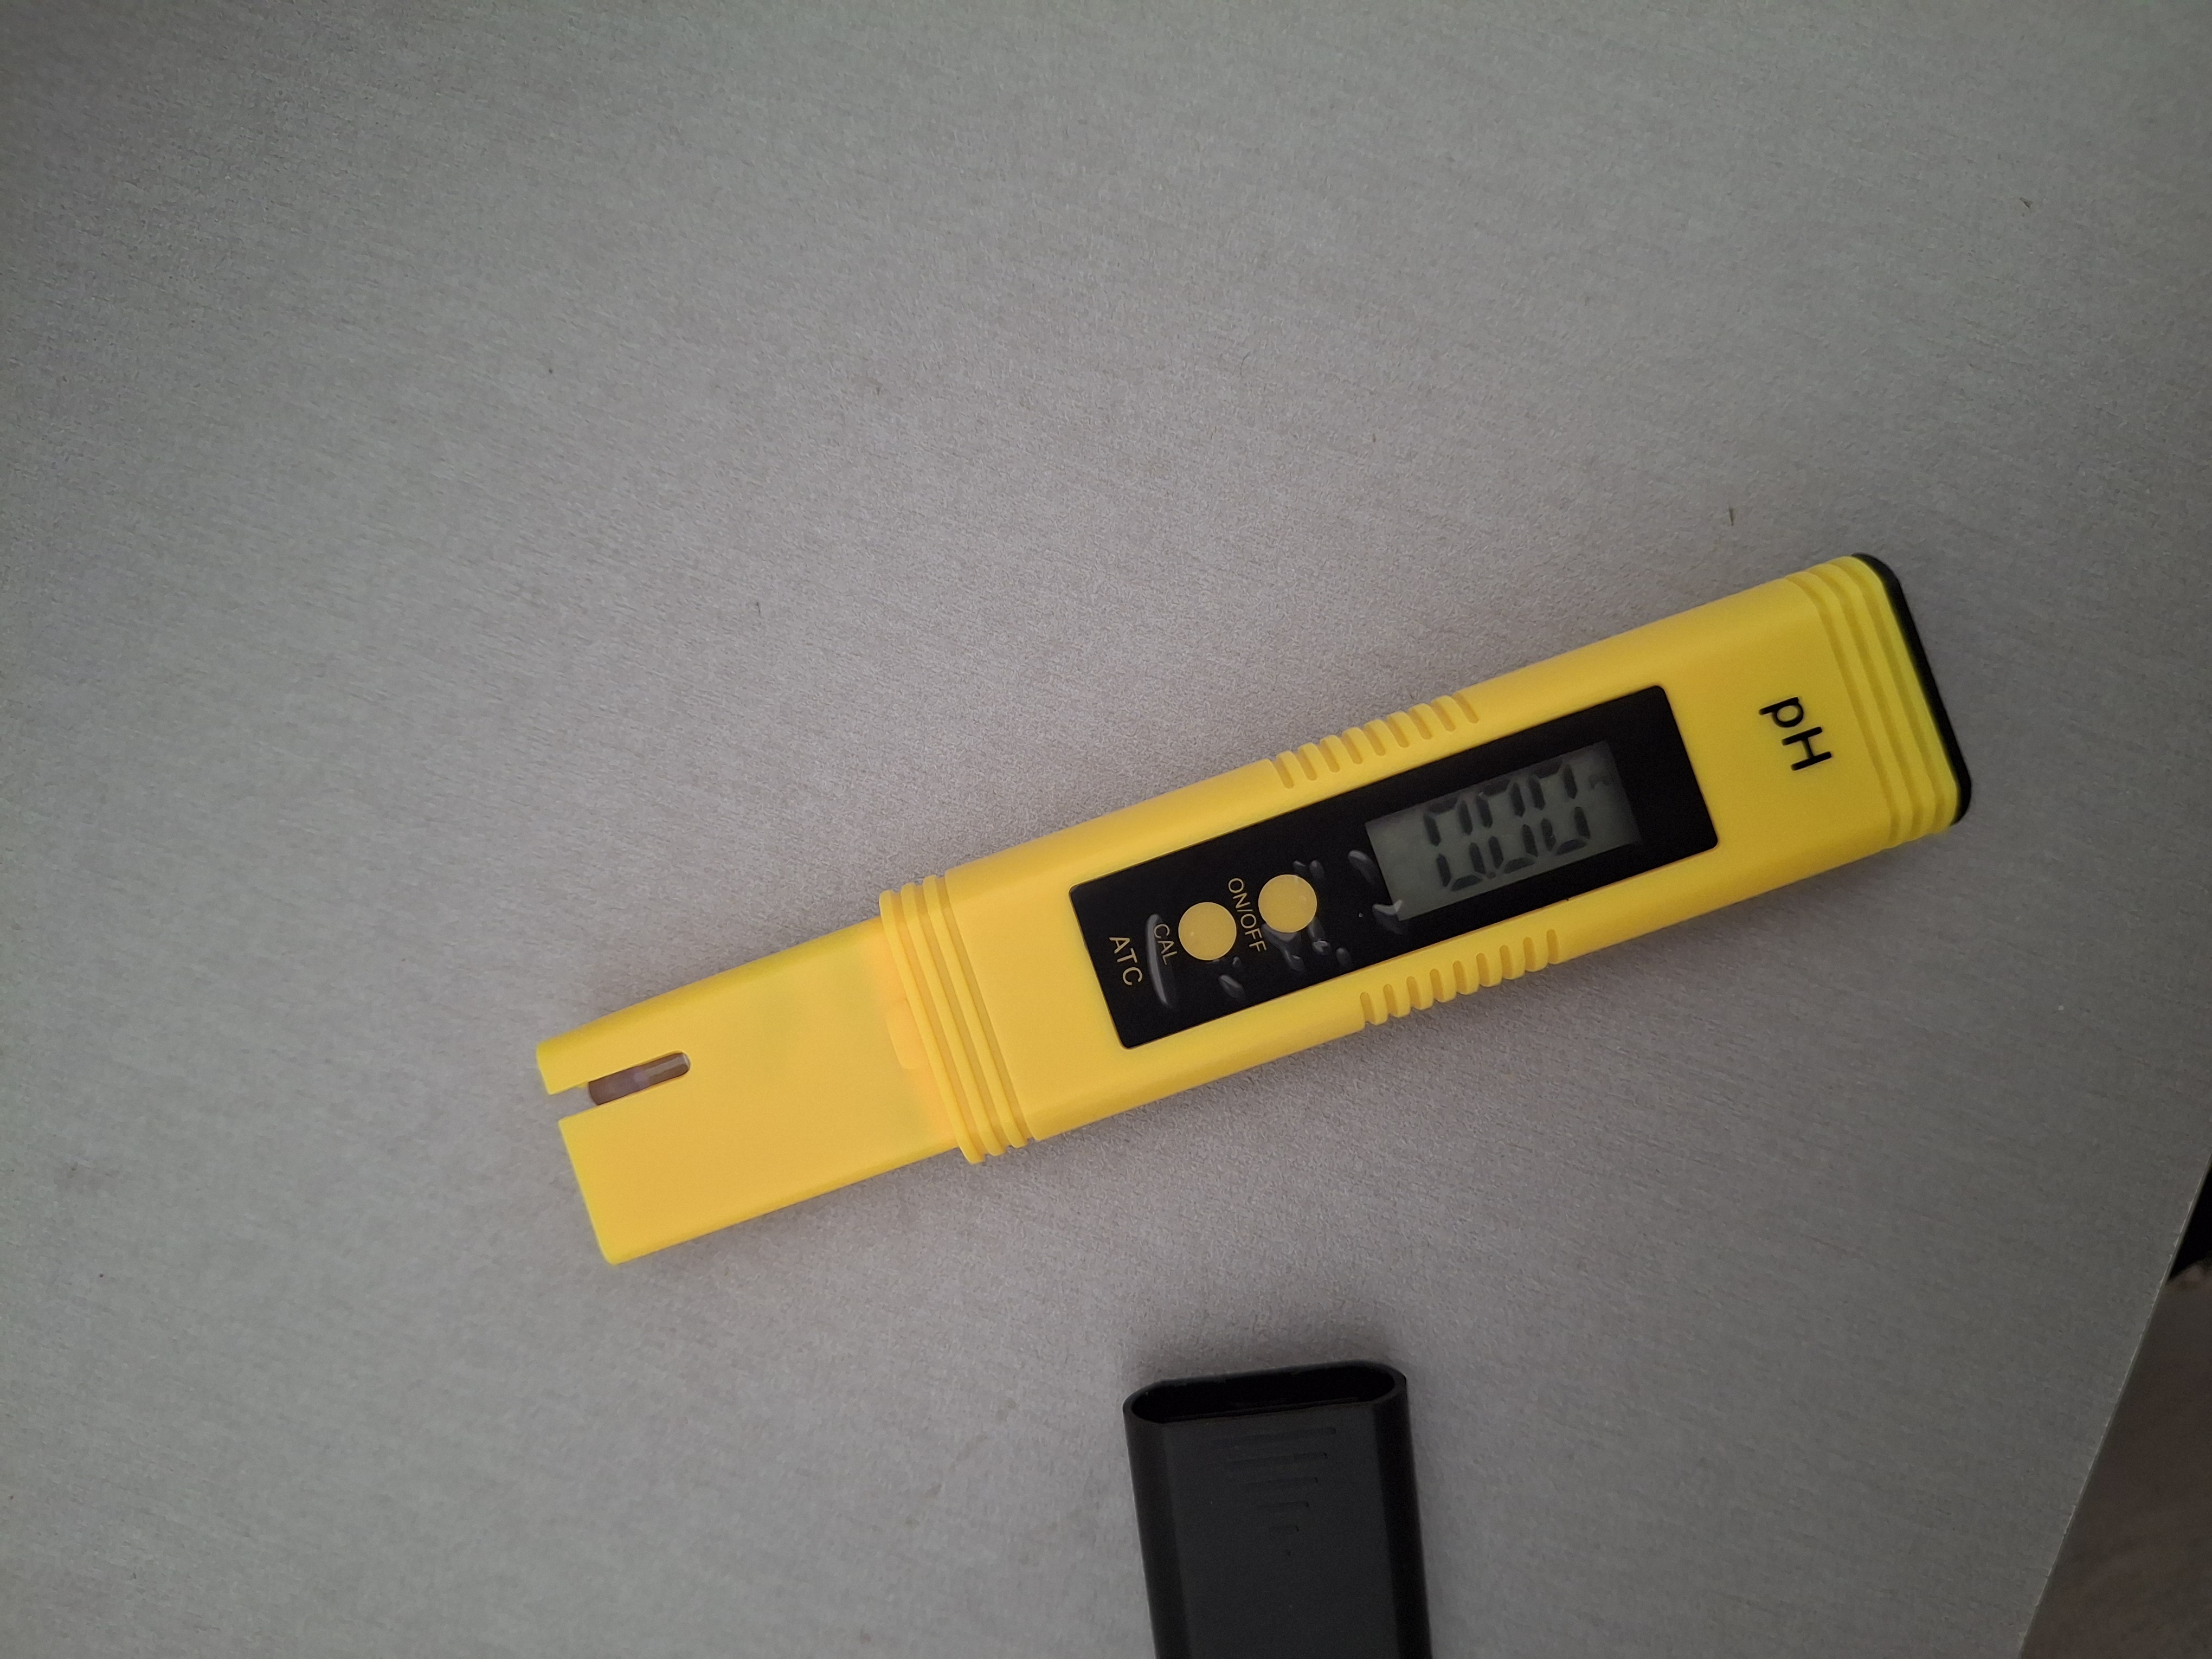
\includegraphics[width=0.5\textwidth]{./Figures/mesurador.png}
\caption{Mesurador de pH}
\label{fig:foto}
\end{figure}

Quan ja tenia tot el material necessari, vaig començar amb l’experimentació. Tots els passos i resultats els anotava en una llibreta que havia comprat especialment per a aquest projecte.

Vaig haver d’investigar com utilitzar correctament les tires, ja que inicialment no en coneixia el procediment. Després de veure alguns vídeos i consultar diverses fonts, vaig aprendre que calia submergir la tira durant un segon i retirar-la immediatament. En aquest punt em vaig trobar amb un dubte: hi havia qui deixava assecar la tira al sol i qui no. Davant aquesta contradicció, vaig decidir provar tots dos mètodes per comprovar si hi havia diferències entre ells.

La decisió de provar amb i sense llum solar també venia d’una contradicció en les instruccions del paquet. A l’envàs exterior (en anglès), s’indicava que les tires no havien de tenir contacte amb la llum solar directa. Però, sorprenentment, a l’interior —també en anglès— les instruccions deien el contrari: que s’havien d’assecar al sol. Aquesta incoherència em va portar a fer l’experiment de les dues maneres.

Després d’assecar la tira durant 60 segons, ja es podien observar els colors que indicaven la presència i concentració de cada compost. Segons la intensitat del color, es podia determinar el valor aproximat. Ara bé, aquest sistema presentava una dificultat: els colors no sempre eren clars ni fàcils de comparar amb la guia de referència, cosa que feia que els resultats fossin sempre aproximats i no totalment precisos.

Abans de començar oficialment amb les mesures, vaig organitzar totes les mostres. L’aigua de l’aixeta la vaig guardar en una ampolla de plàstic degudament etiquetada per no confondre-la amb altres mostres. També vaig col·locar etiquetes a gairebé tot: les tires segons si s’assecarien amb o sense llum solar, els gots amb les diferents aigües, i les tires de l’institut.
\begin{figure}[H]
\centering
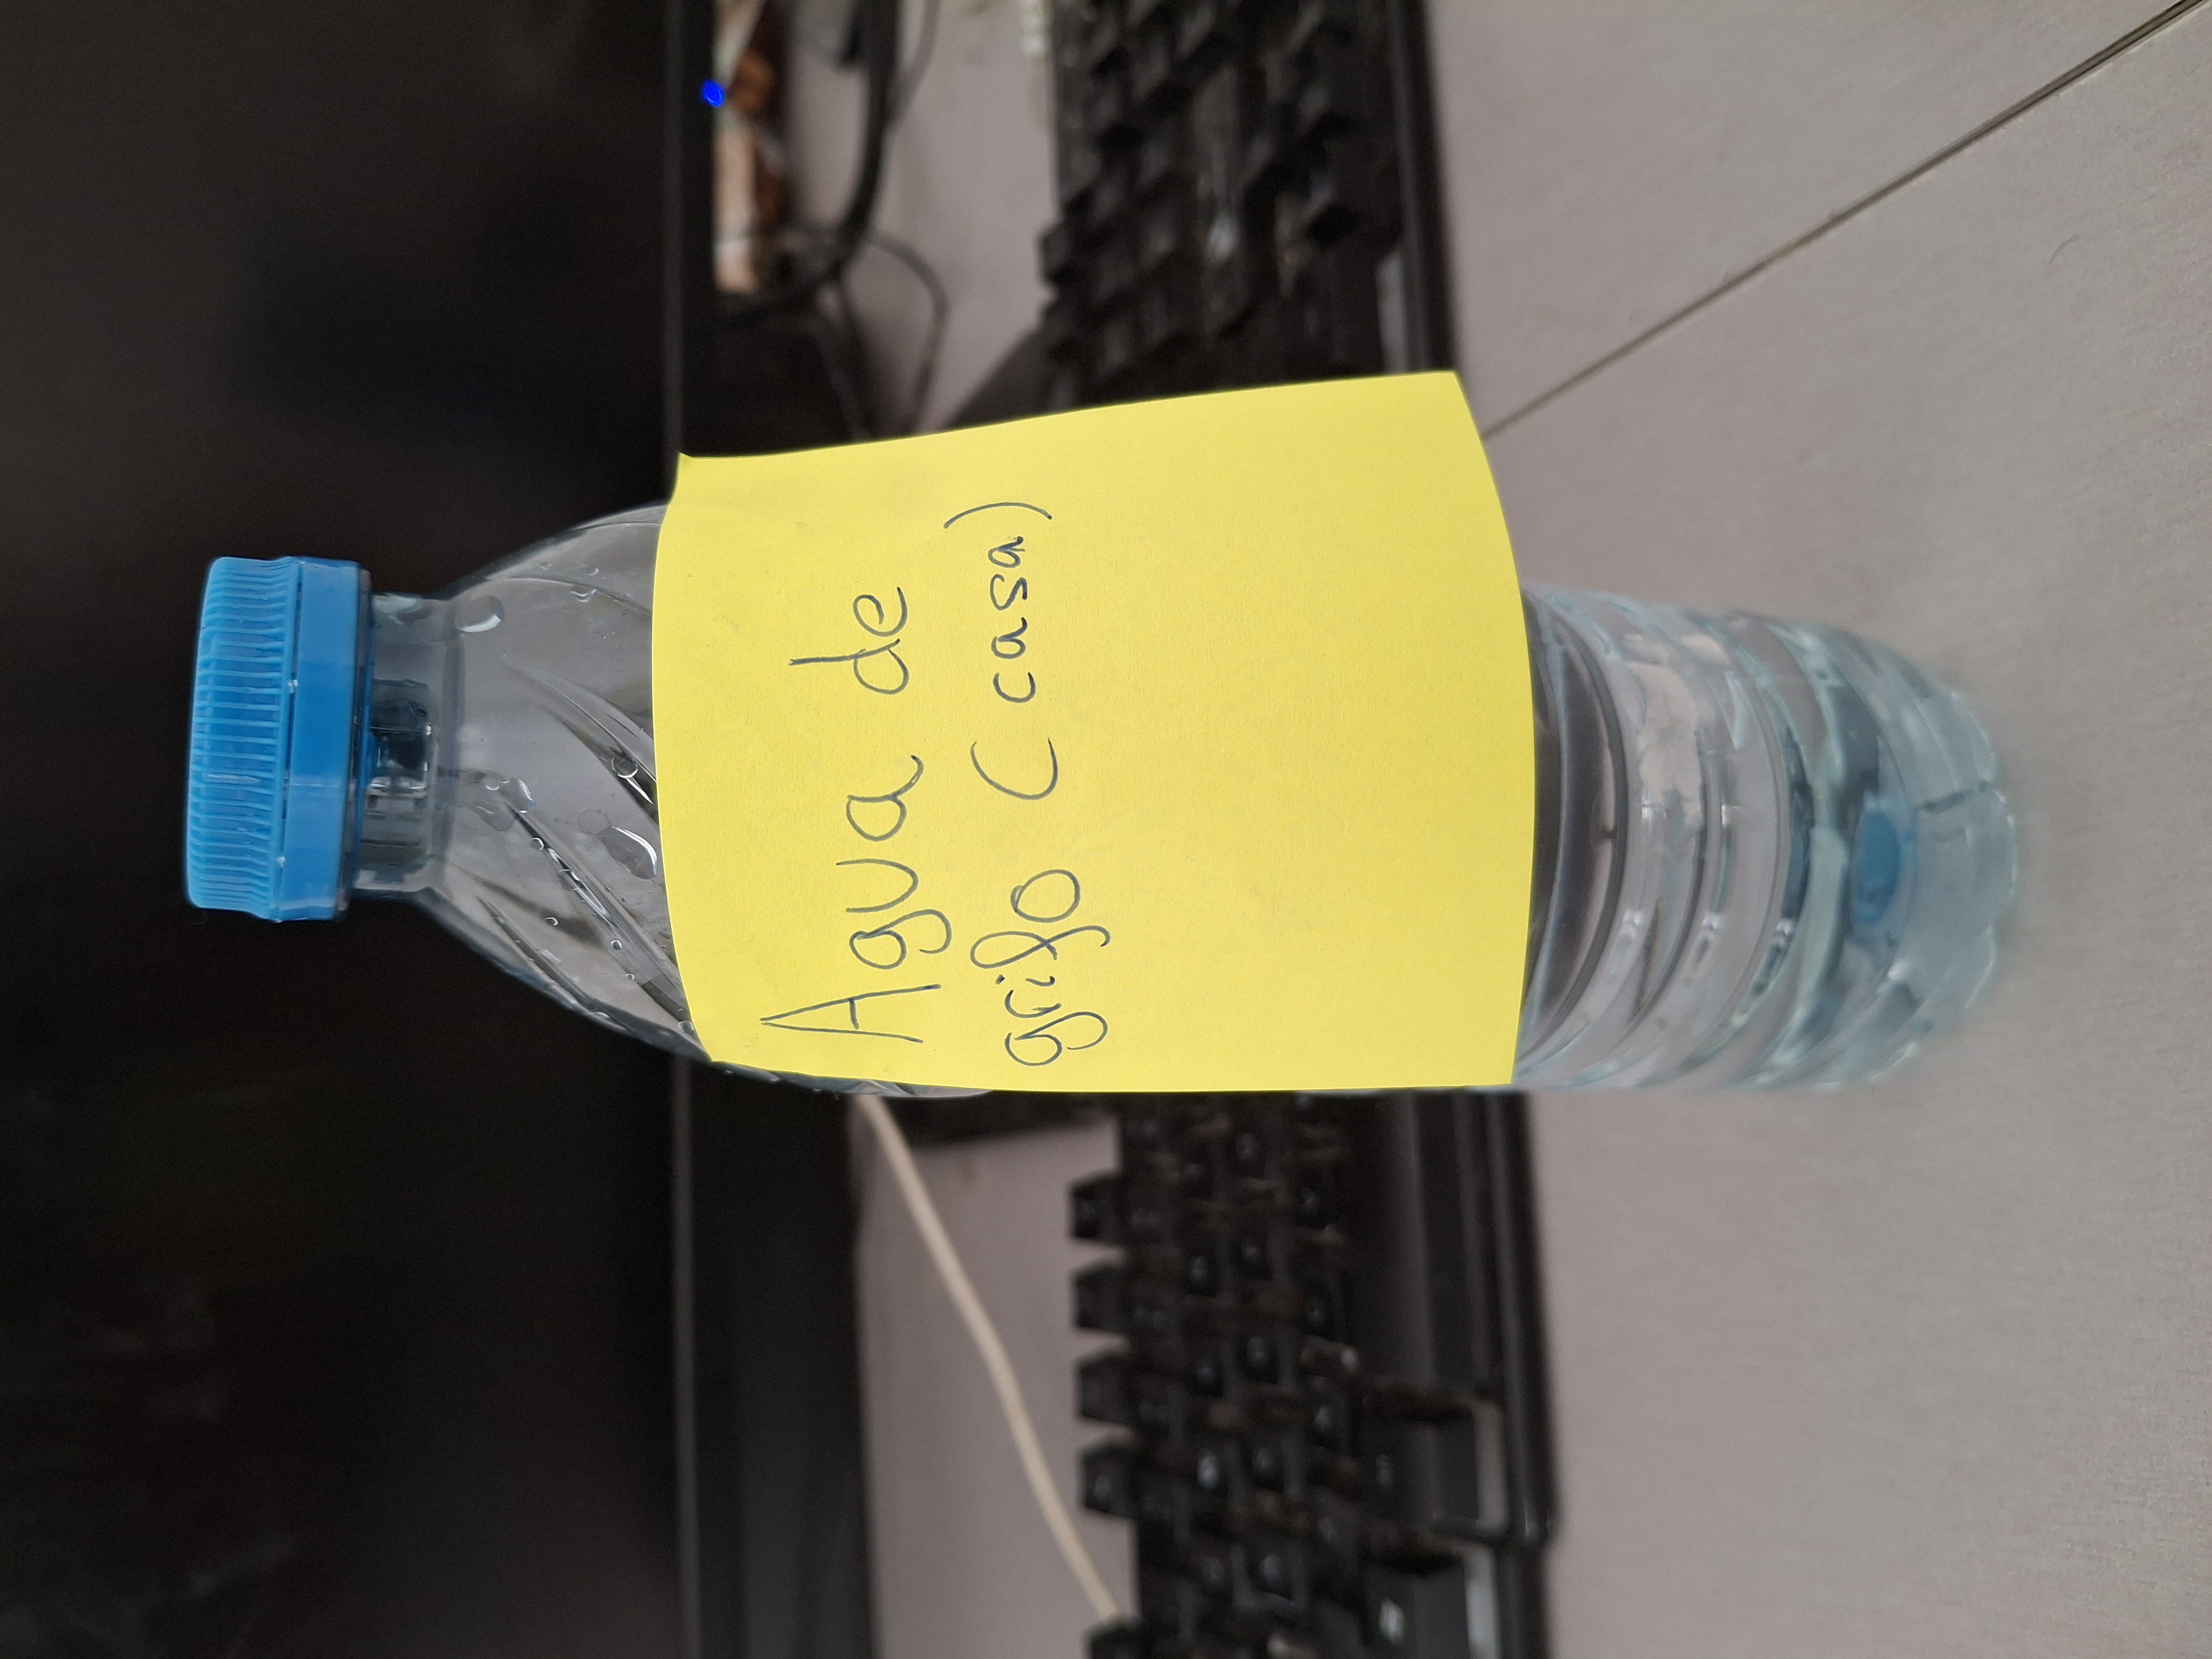
\includegraphics[width=0.5\textwidth, angle=270]{./Figures/aguadecasa.png}
\caption{Aigua de casa meva}
\label{fig:foto}
\end{figure}

\begin{figure}[H]
\centering
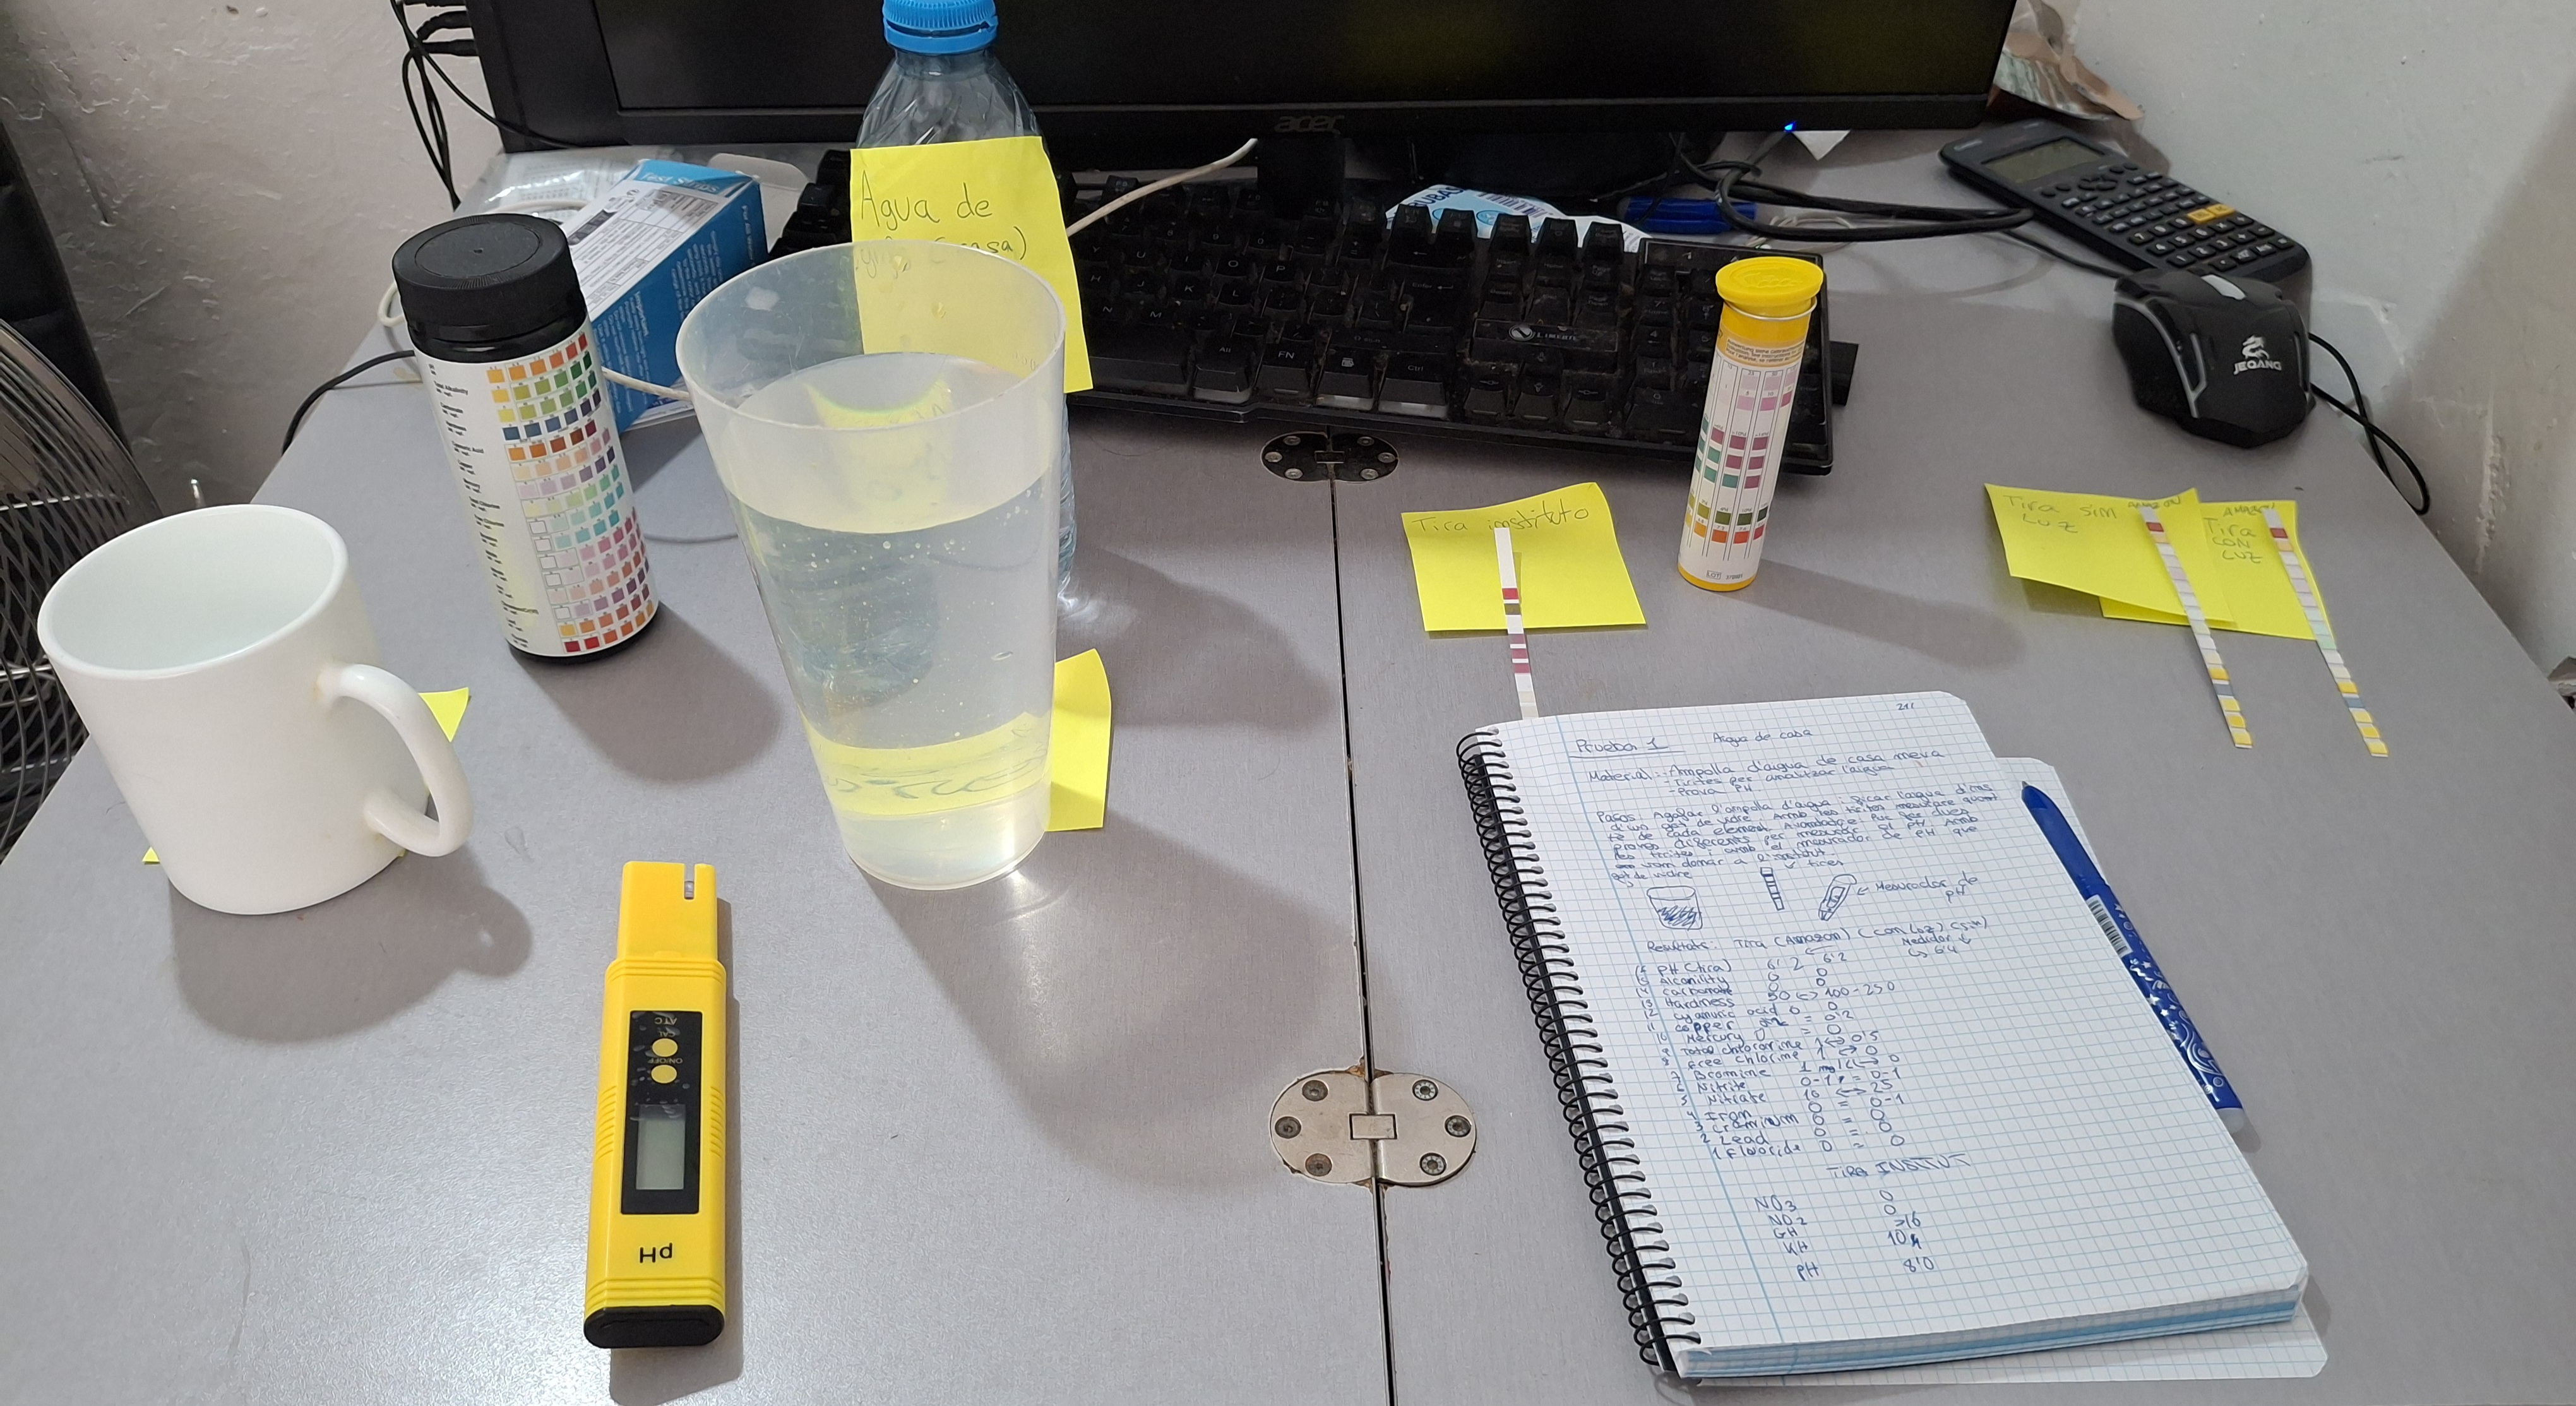
\includegraphics[width=1\textwidth, angle=0]{./Figures/expe.png}
\caption{Pre-experiment }
\label{fig:foto}
\end{figure}

Els passos que vaig seguir van ser els següents: en un got hi vaig posar l’aigua de l’aixeta i en un altre, l’aigua destil·lada. Vaig començar utilitzant les tires d’Amazon, però em vaig adonar que els components químics estaven escrits en anglès, així que vaig haver-los de traduir per saber què estava mesurant i poder anotar-ho a la llibreta.

Primer vaig fer la prova amb les tires exposades a la llum solar. A continuació, vaig repetir l’experiment amb una tira nova, però aquesta vegada sense exposició solar. A continuació, mostro els resultats obtinguts:

\begin{table}[H]
\centering
\caption{Comparació entre els valors experimentals}
\resizebox{\textwidth}{!}{
\begin{tabular}{|l|c|p{2.2cm}|p{2.2cm}|c|}
\hline
Components en Anglès & Components en Català & Resultats amb llum solar en mg/L & Resultats sense llum solar en mg/L & Mesurador de pH \\
\hline
pH    & pH    & 6.2      & 6.2 & 7.21\\
\hline
Total alkalinity    & Alcalinitat total(CaCO$_3$)    & 0    & 0 &---\\
\hline
Carbonate    & Carbonat     & 0      & 0 & --- \\
\hline
Hardness    & Duresa (GH)   & 50          & 175  &---\\
\hline
Cyanuric acid    & Àcid cianúric    & 0     & 0  & ---\\
\hline
Copper    &  Coure    & 0.2       & 0.1 &---\\
\hline
Mercury  & Mercuri    & 0      & 0  &---\\
\hline
Total chlorine  &  Clor total     & 1     & 0.5 & --- \\
\hline
Free chlorine    & Clor lliure    & 1      & 0  &---\\
\hline
Bromine    & Brom  & 1      & 0  &---\\
\hline
Nitrite    & Nitrit    & 0.5       & 0.5 & ---\\
\hline
Nitrate    & Nitrat (NO$_3^-$)    & 10        & 25  &---\\
\hline
Iron   & Ferro    & 0      & 0.5  & ---\\
\hline
Chromium / Cr(VI)    & Crom (VI)   & 0      & 0  &---\\
\hline
Lead    & Plom   & 0     & 0  &---\\
\hline
Fluoride    & Fluorur (F$^-$)    & 0      & 0   &---\\
\hline
\end{tabular}
}
\label{tab:comparacio_dades}
\end{table}

Tal com es pot veure, en general no hi ha diferències molt grans entre fer la prova amb o sense exposició solar. Tot i així, hi ha alguns casos destacats. Per exemple, la duresa presenta un salt important: 50 mg/L amb llum solar, i 175 mg/L sense. També els nitrats mostren una diferència significativa: 10 mg/L amb sol i 25 mg/L sense. Altres compostos com el ferro o el clor total mostren variacions més lleus, però també notables. En canvi, el clor lliure apareix amb 1 mg/L en la tira exposada al sol, i 0 mg/L en la que no hi ha estat.

Un cas especialment curiós ha estat el del pH, ja que els tres mètodes emprats han coincidit en un valor de 6.2. Inicialment pensava que aquest seria un dels valors més variables.

Les dades reals de l’aigua les vaig consultar a la web d’Aigües de Barcelona. Un cop feta la comparació, aquests són els resultats obtinguts amb les dues tires, tant amb exposició solar com sense.

\begin{table}[H]
\centering
\caption{Comparació entre els valors experimentals i els oficials de l'aigua de l'aixeta (amb exposició solar)}
\resizebox{\textwidth}{!}{
\begin{tabular}{|l|c|c|c|p{4.2cm}|}
\hline
\textbf{Paràmetre} & \textbf{Valor experimental} & \textbf{Valor oficial} & \textbf{Unitats} & \textbf{Comentari} \\
\hline \hline
pH & 6,2 & 7,2 & unitats pH & Inferior al valor oficial; aigua més àcida. \\
\hline
Alcalinitat total & 0 & 182 & mg CaCO$_3$/L & Valor experimental probablement incorrecte. \\
\hline
Carbonats & 0 & --- & mg /L & Informació no proporcionada. \\
\hline
Duresa total & 50 & 271 & mg GH /L & Molt inferior al valor oficial. \\
\hline
Nitrat & 10 & 7,17 & mg NO$_3^-$ /L & Lleugerament superior; dins de marges acceptables. \\
\hline
Nitrit & 0.5 & ---& mg /L & Informació no proporcionada. \\
\hline
Clor total & 1 & --- & mg/L & Valor comú en aigües potables. \\
\hline
Clor lliure & 1 & --- & mg/L & Idèntic al valor anterior. \\
\hline
Ferro & 0 & --- & mg/L & No detectat; valor desitjable. \\
\hline
Fluorur & 0 & $<$0,2 & mg F$^-$ /L & Coincideix amb el límit inferior. \\
\hline
Crom (VI) & 0 & --- & mg/L & No present, tal com és recomanable. \\
\hline
Plom & 0 & --- & mg/L & Absent, com hauria de ser. \\
\hline
Àcid cianúric & 0 & --- & mg/L & No rellevant en aigua potable. \\
\hline
Coure & 0,2 & --- & mg/L & Dins dels límits legals. \\
\hline
Brom & 1 & --- & mg/L & No habitual en aigua potable. \\
\hline
Mercuri & 0 & --- & mg/L & No present; correcte. \\
\hline
\end{tabular}%
}
\label{tab:comparacio_aigua_amb_sol}
\end{table}





\begin{table}[H]
\centering
\caption{Comparació entre els valors experimentals i els oficials de l'aigua de l'aixeta (sense exposició solar)}
\resizebox{\textwidth}{!}{%
\begin{tabular}{|l|c|c|c|p{4.2cm}|}
\hline
\textbf{Paràmetre} & \textbf{Valor experimental} & \textbf{Valor oficial} & \textbf{Unitats} & \textbf{Comentari} \\
\hline \hline
pH & 6,2 & 7,2 & unitats pH & Inferior al valor oficial; aigua més àcida. \\
\hline
Alcalinitat total & 0 & 182 & mg CaCO$_3$/L & Valor experimental probablement incorrecte. \\
\hline
Carbonats & 0 & --- & mg /L & Informació no proporcionada. \\
\hline
Duresa total & 175 & 271 & mg GH/L & Millor aproximació al valor real que abans. \\
\hline
Nitrat & 25 & 7,17 & mg NO$_3^-$ /L & Molt lluny al valor oficial. \\
\hline
Nitrit & 0.5 & ---& mg /L & Informació no proporcionada. \\
\hline
Clor total & 0,5 & --- & mg/L & Ligerament inferior a la prova amb sol. \\
\hline
Clor lliure & 0 & --- & mg/L & Idèntic al total; valor típic. \\
\hline
Ferro & 0.5 & --- & mg/L & Ligerament superior al valor amb sol; no hauria de tenir. \\
\hline
Fluorur & 0 & $<$0,2 & mg F$^-$ /L & Coincideix amb el valor esperat. \\
\hline
Crom (VI) & 0 & --- & mg/L & No present. \\
\hline
Plom & 0 & --- & mg/L & No detectat; adequat. \\
\hline
Àcid cianúric & 0 & --- & mg/L & No rellevant; igual que en la prova anterior. \\
\hline
Coure & 0,1 & --- & mg/L & Ligerament inferior al valor amb sol; dins límits. \\
\hline
Brom & 0 & --- & mg/L & No detectat en aquest cas. \\
\hline
Mercuri & 0 & --- & mg/L & No detectat; correcte. \\
\hline
\end{tabular}%
}
\label{tab:comparacio_aigua_sense_sol}
\end{table}

Com es pot veure, les tires no han encertat en alguns dels valors; en d’altres sí. Tot i això, el problema principal ha estat que les tires no mesuren exactament els mateixos paràmetres que apareixen a la web d’Aigües de Barcelona. Per tant, no es pot fer una comparació directa de tots els valors, sinó que ens hem de limitar només als que coincideixen en ambdós casos.

També cal aclarir que hi ha determinats paràmetres que no es tenen en compte en l’aigua potable, i això fa que sigui impossible comparar-los. El que més m’ha sorprès, però, ha estat la comparació següent:

\begin{table}[H]
\centering
\caption{Comparació entre els valors experimentals i els oficials de l'aigua de l'aixeta (amb el mesurador de pH)}
\resizebox{\textwidth}{!}{%
\begin{tabular}{|c|c|c|}
\hline
\textbf{Paràmetre} & \textbf{Valor experimental} & \textbf{Valor oficial} \\
\hline \hline
pH & 7.21 & 7,2 \\
\hline
\end{tabular}
}
\label{tab:comparacio_aigua_sense_sol}
\end{table}

Tal com es pot apreciar a la taula, el nivell de pH coincideix amb el valor oficial. Aquesta conclusió em va donar molta confiança a l’hora de fer mesures amb el mesurador digital, ja que, com he comentat anteriorment, és molt més fiable que qualsevol tira reactiva, ja que proporciona un valor exacte i no una aproximació basada en colors.

Així va ser el meu primer experiment. No puc dir que n’hagi sortit del tot satisfet, ja que he tingut força decepcions, però també algunes alegries. Com que era el primer cop que ho feia, he après dels meus errors, ara sé què he de fer i què no la pròxima vegada, i tot plegat m’ha ajudat a organitzar-me molt millor. Una cosa és imaginar com serà tot i una altra molt diferent és viure-ho. Es podria dir que ha estat com una clatellada de realitat. Però, en el fons, aquesta és la gràcia de l’experimentació.
